\documentclass{beamer}
\usepackage{amsfonts,amsmath,oldgerm}
\usetheme{sintef}

\newcommand{\testcolor}[1]{\colorbox{#1}{\textcolor{#1}{test}}~\texttt{#1}}

\usefonttheme[onlymath]{serif}

% Assicurati di avere un'immagine in assets/background o commenta la riga seguente
\titlebackground*{assets/background}

\newcommand{\hrefcol}[2]{\textcolor{cyan}{\href{#1}{#2}}}

\title{Parallel Morphological Image Processing}
\subtitle{Accelerating morphological operations via C++17 and OpenMP}
\author{\href{mailto:davide.lombardi2@edu.unifi.it}{Davide Lombardi}}
\date{July 20, 2026}

\begin{document}
\maketitle

% --- SLIDE 1 ---
\begin{frame}{Introduction}
  \begin{itemize}
    \item \textbf{Mathematical Morphology:} framework for geometric feature extraction and image restoration
    \item \textbf{Targeted Operations:}
      \begin{itemize}
        \item \textit{Fundamental:} Erosion, Dilation
        \item \textit{Compound:} Opening, Closing
      \end{itemize}
    \item \textbf{Goal:} resolve computational bottlenecks in high-resolution image processing
    \item \textbf{Technology Stack:} \texttt{C++17} and \texttt{OpenMP} for thread orchestration
    \item \textbf{Dataset \& Benchmarks:} BSDS500
      \begin{itemize}
        \item Preliminary grayscale conversion
        \item 2.0x and 4.0x upscaling to evaluate scalability
      \end{itemize}
  \end{itemize}
\end{frame}

% --- SLIDE 2 ---
\begin{frame}{Context \& Architectural Limits}
  \begin{columns}
    \begin{column}{0.45\textwidth}
      \begin{block}{Operator Logic}
        \begin{itemize}
          \item \textbf{Erosion:} minimum extraction in a defined spatial neighborhood
          \item \textbf{Dilation:} maximum extraction in a defined spatial neighborhood
          \item \textbf{Opening:} Erosion followed by Dilation
          \item \textbf{Closing:} Dilation followed by Erosion
        \end{itemize}
      \end{block}
    \end{column}
    \begin{column}{0.55\textwidth}
      \begin{colorblock}[white]{sintefred}{The Memory Wall \& Complexity}
        \begin{itemize}
          \item Naive execution with 2D stencils strictly bound by $\mathcal{O}(M \times N \times K^2)$ complexity
          \item \textbf{Compound operations} implemented sequentially (double-pass approach)
          \item \textbf{System Overhead:} destruction of \textit{temporal locality} and cache saturation between passes
        \end{itemize}
      \end{colorblock}
    \end{column}
  \end{columns}
\end{frame}

% --- SLIDE 3 ---
\begin{frame}{Hardware Optimization: Pixel-Level Parallelism}
  \begin{itemize}
    \item Spatial stencil processing is inherently independent for each pixel 
    \item \textbf{Loop Collapsing (\texttt{collapse(2)}):} logical fusion of X and Y image axes
      \begin{itemize}
        \item Expands the iteration space and distributes workload with fine granularity
        \item Prevents \textit{thread starvation} at boundaries
      \end{itemize}
    \item \textbf{Memory Safety (\texttt{default(none)}):} forced explicit scoping
      \begin{itemize}
        \item Thread-local allocation for temporary variables (e.g., \texttt{min\_val})
        \item Avoids synchronization overhead (zero locks or atomics) in the critical loop
      \end{itemize}
    \item \textbf{Static Scheduling (\texttt{schedule(static)}):} deterministic work distribution
      \begin{itemize}
        \item Zero runtime overhead, ideal for uniform per-pixel workloads (invariant $K \times K$ footprint)
        \item \textit{Note:} dynamic chunking later explored
      \end{itemize}
  \end{itemize}
\end{frame}

% --- SLIDE 4 ---
\begin{frame}{Algorithmic Optimization: 1D Separable Kernels}
  \begin{itemize}
    \item \textbf{The Dominant Lever:} decomposition of the $K \times K$ stencil into two independent passes (Horizontal $\rightarrow$ Vertical)
    \item \textbf{Computational Reduction:} transition from $\mathcal{O}(K^2)$ to linear $\mathcal{O}(2K)$
      \begin{itemize}
        \item Using a $15 \times 15$ kernel, base operations per pixel drop from 225 to just 30
      \end{itemize}
  \end{itemize}
  
  \begin{block}{The Architectural Trade-off (Cache Asymmetry)}
    \begin{itemize}
      \item \textbf{Horizontal Pass:} highly efficient, exploits prefetching and RAM \textit{spatial locality} (row-major layout)
      \item \textbf{Vertical Pass:} introduces severe cache misses, forcing the memory bus to work column-wise
    \end{itemize}
  \end{block}
\end{frame}

% --- SLIDE 5 ---
\begin{frame}{Producer-Consumer Pipeline}
  \begin{itemize}
    \item \textbf{The Fork-Join Problem:} pure 1D Closing requires 4 global passes, doubling heap footprint and introducing strict synchronization barriers
    \item \textbf{OpenMP Pipeline Design:} 
      \begin{itemize}
        \item Single partitioned parallel region where half the threads act as Producers and half as Consumers
        \item Fine-grained chunk synchronization via \texttt{PaddedFlag} array to eliminate false sharing
      \end{itemize}
    \item \textbf{Architectural Benefits:} execution overlap and keeps pixels in cache (\textit{temporal locality})
  \end{itemize}
\end{frame}



\begin{chapter}[assets/background]{maincolor}{Performance Results}
\end{chapter}
% --- SLIDE 7 ---
\begin{frame}{Strong \& Weak Scalability Analysis}
  \begin{columns}
    \begin{column}{0.5\textwidth}
      \begin{figure}
          \centering
          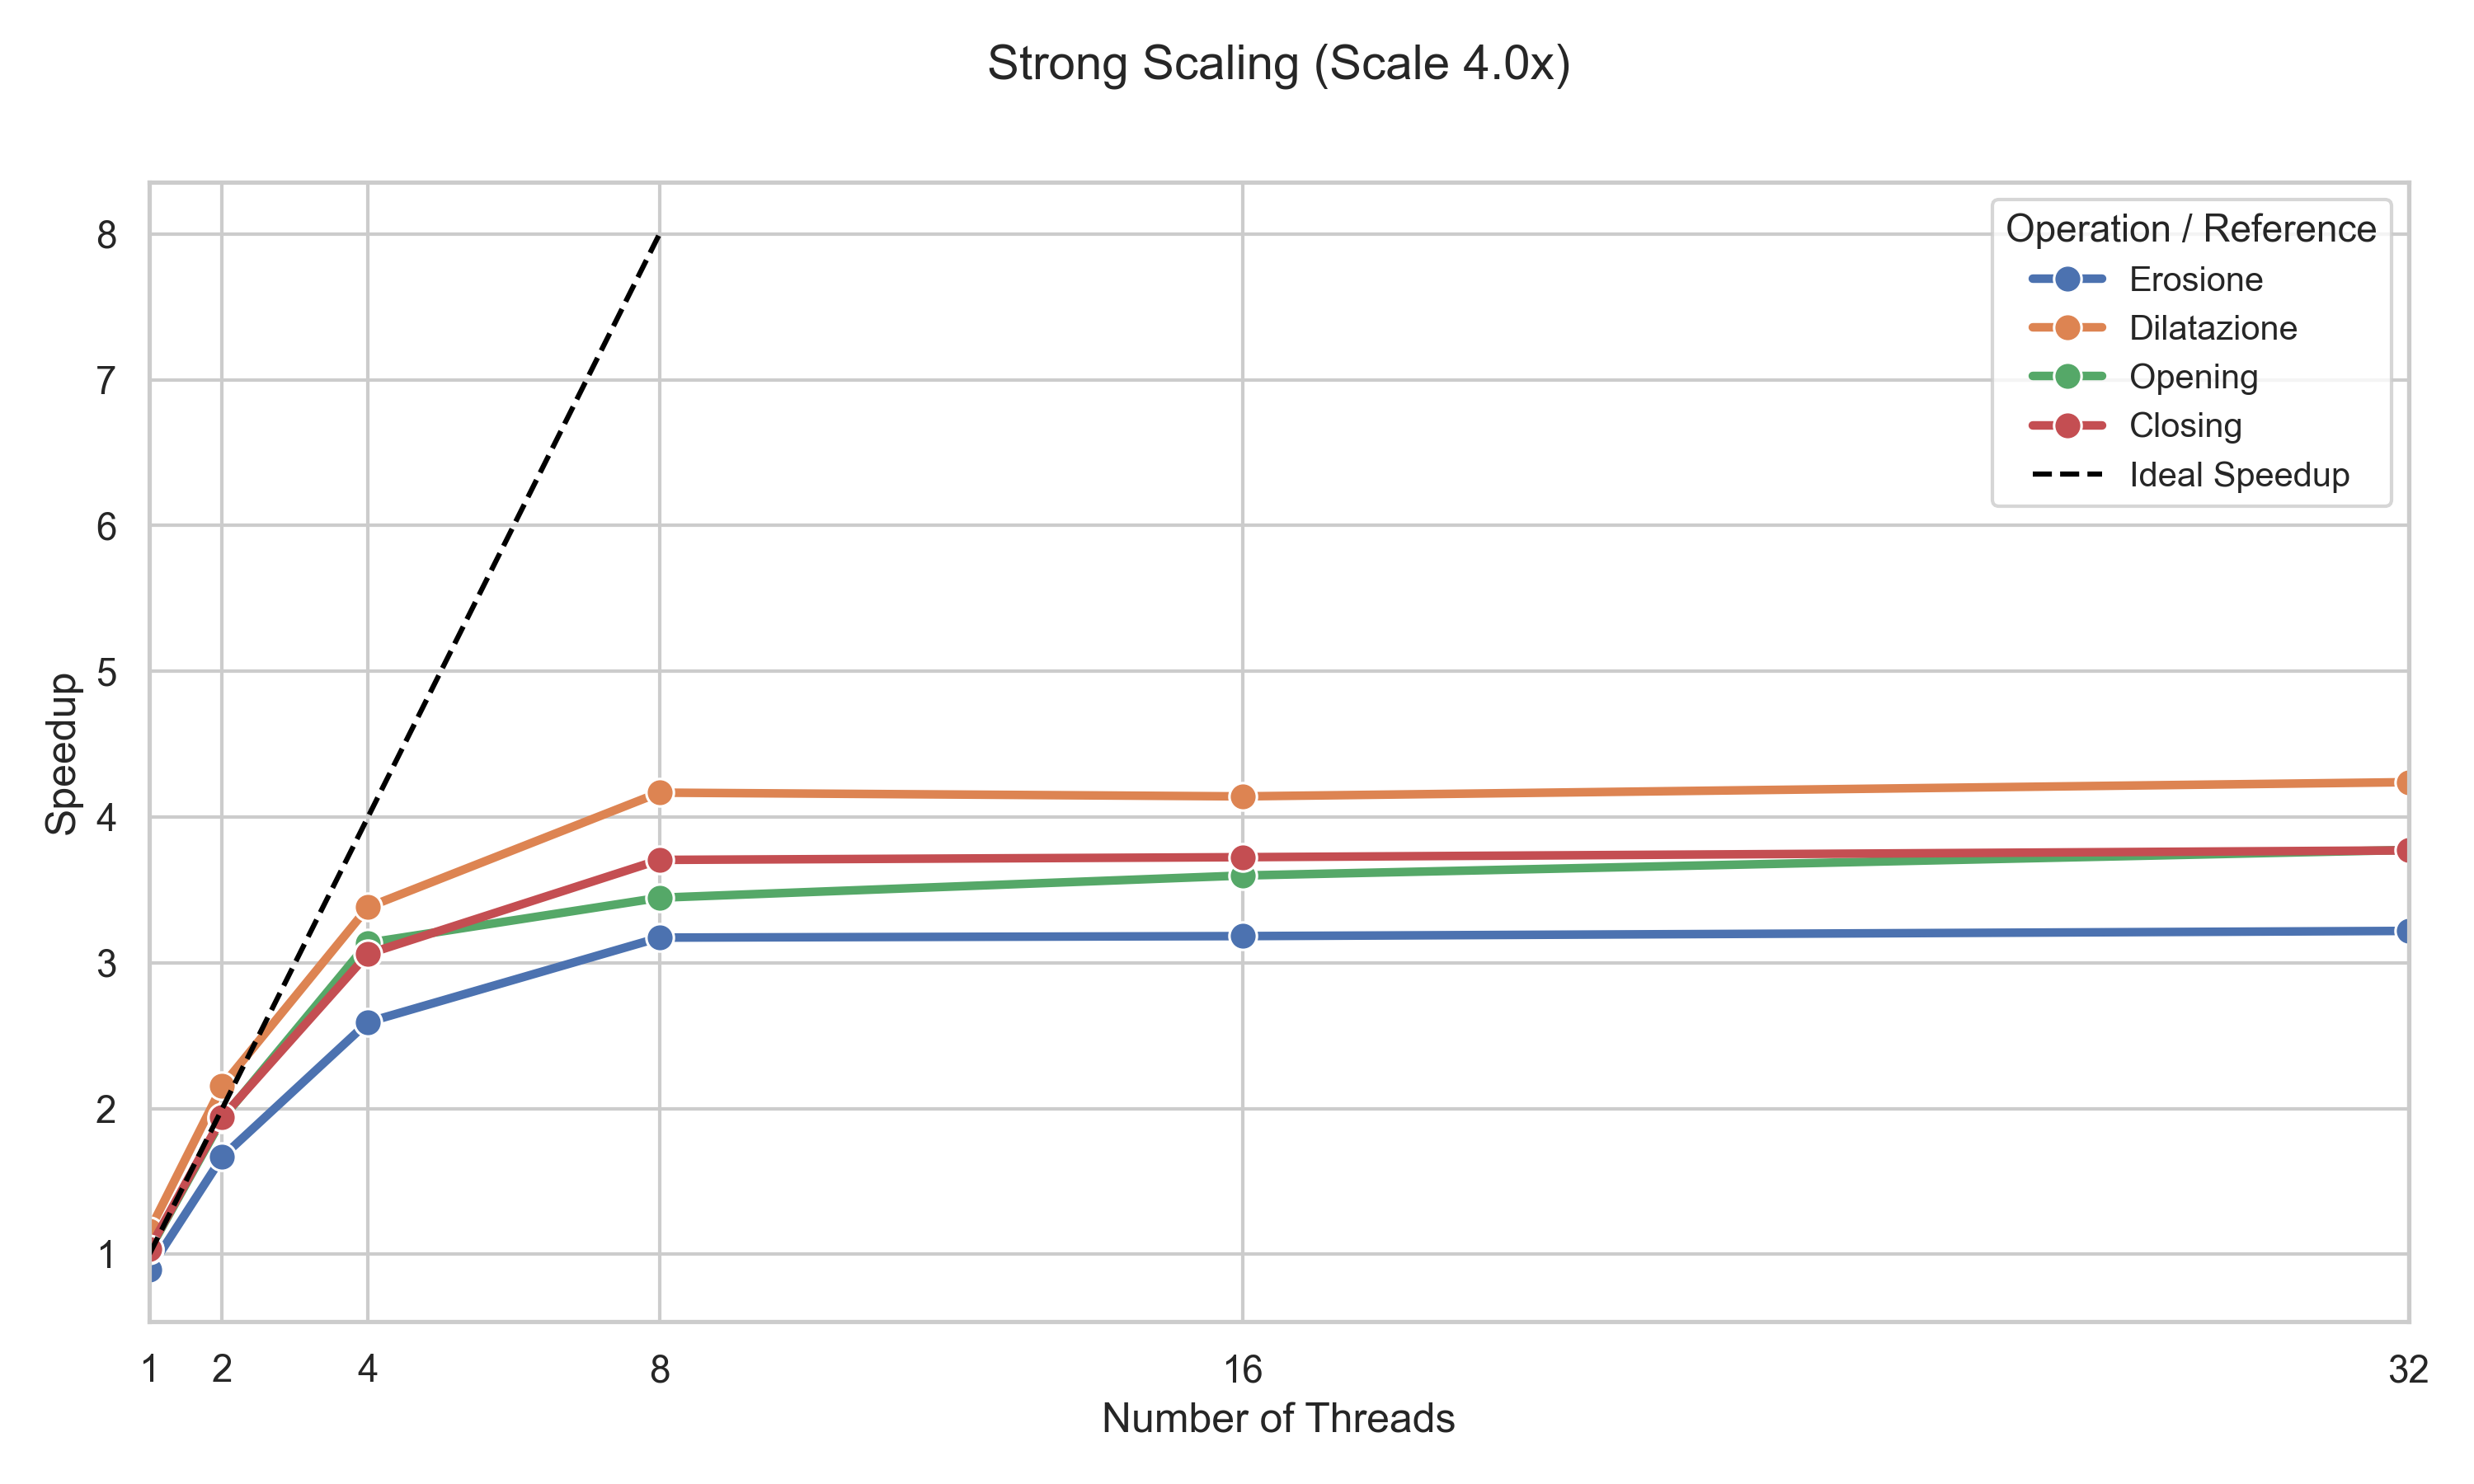
\includegraphics[width=0.85\textwidth]{img/strong_scaling.png}
          \caption{Strong Scaling (Fixed Workload)}
      \end{figure}
      \vspace{-0.3cm}
      \begin{itemize}
          \footnotesize
          \item Asymptotic saturation at \textbf{3.5x--4.0x} with 4 physical cores
          \item Perfectly reflects \textit{Amdahl's Law} (unavoidable pure sequential fraction)
      \end{itemize}
    \end{column}
    \begin{column}{0.5\textwidth}
      \begin{figure}
          \centering
          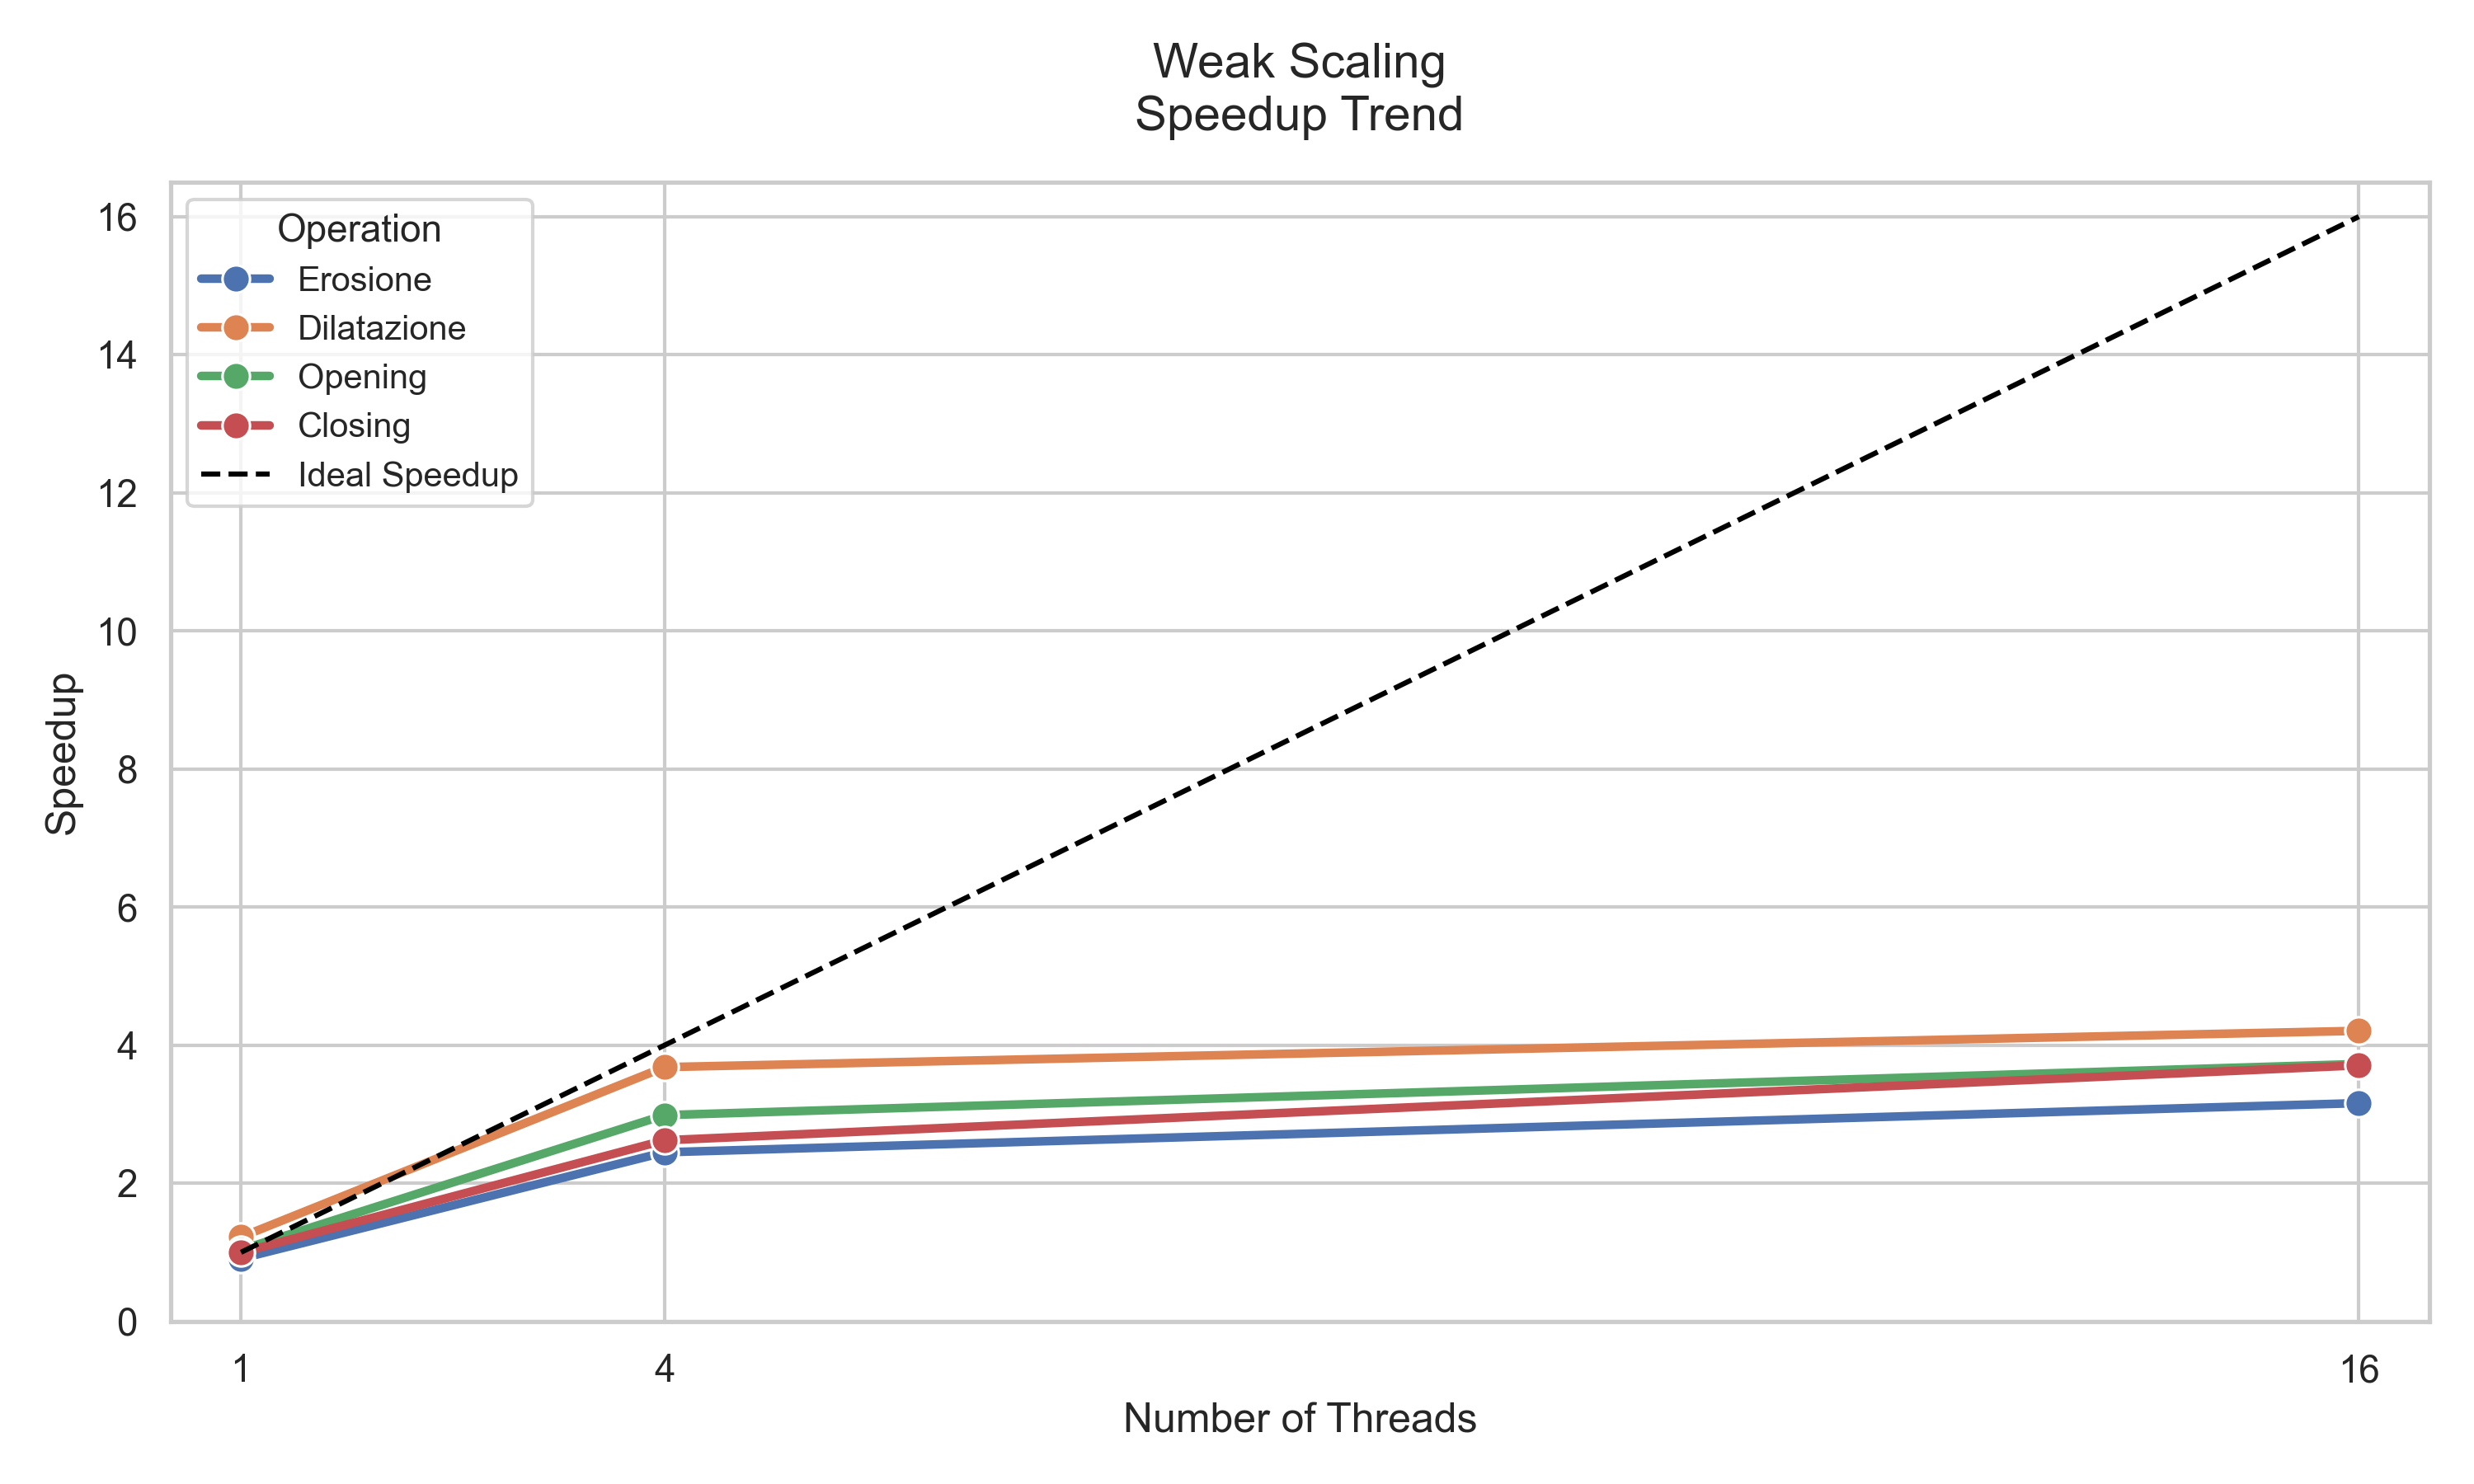
\includegraphics[width=0.85\textwidth]{img/weak_scaling_speedup.png}
          \caption{Weak Scaling (Scaled Workload)}
      \end{figure}
      \vspace{-0.3cm}
      \begin{itemize}
          \footnotesize
          \item Efficiency drops from \textbf{1.0} (1 thread) to \textbf{0.73} (4 threads)
          \item Collapses to \textbf{~0.23} at 16 threads: hyper-threading and RAM bandwidth limits
      \end{itemize}
    \end{column}
  \end{columns}
\end{frame}

% --- SLIDE 8 ---
\begin{frame}{Algorithmic Reduction: 1D vs 2D Performance}
  \begin{columns}
    \begin{column}{0.45\textwidth}
      \begin{itemize}
        \item \textbf{Direct Impact:} transitioning to linear $\mathcal{O}(2K)$ complexity acts as the true performance multiplier
        \item \textbf{Kernel Scaling ($K$):}
          \begin{itemize}
            \item At low $K$ values, the gap is minimal
            \item At high $K$ values, the 2D approach collapses under quadratic load
          \end{itemize}
      \end{itemize}
    \end{column}
    \begin{column}{0.5\textwidth}
      \begin{figure}
          \centering
          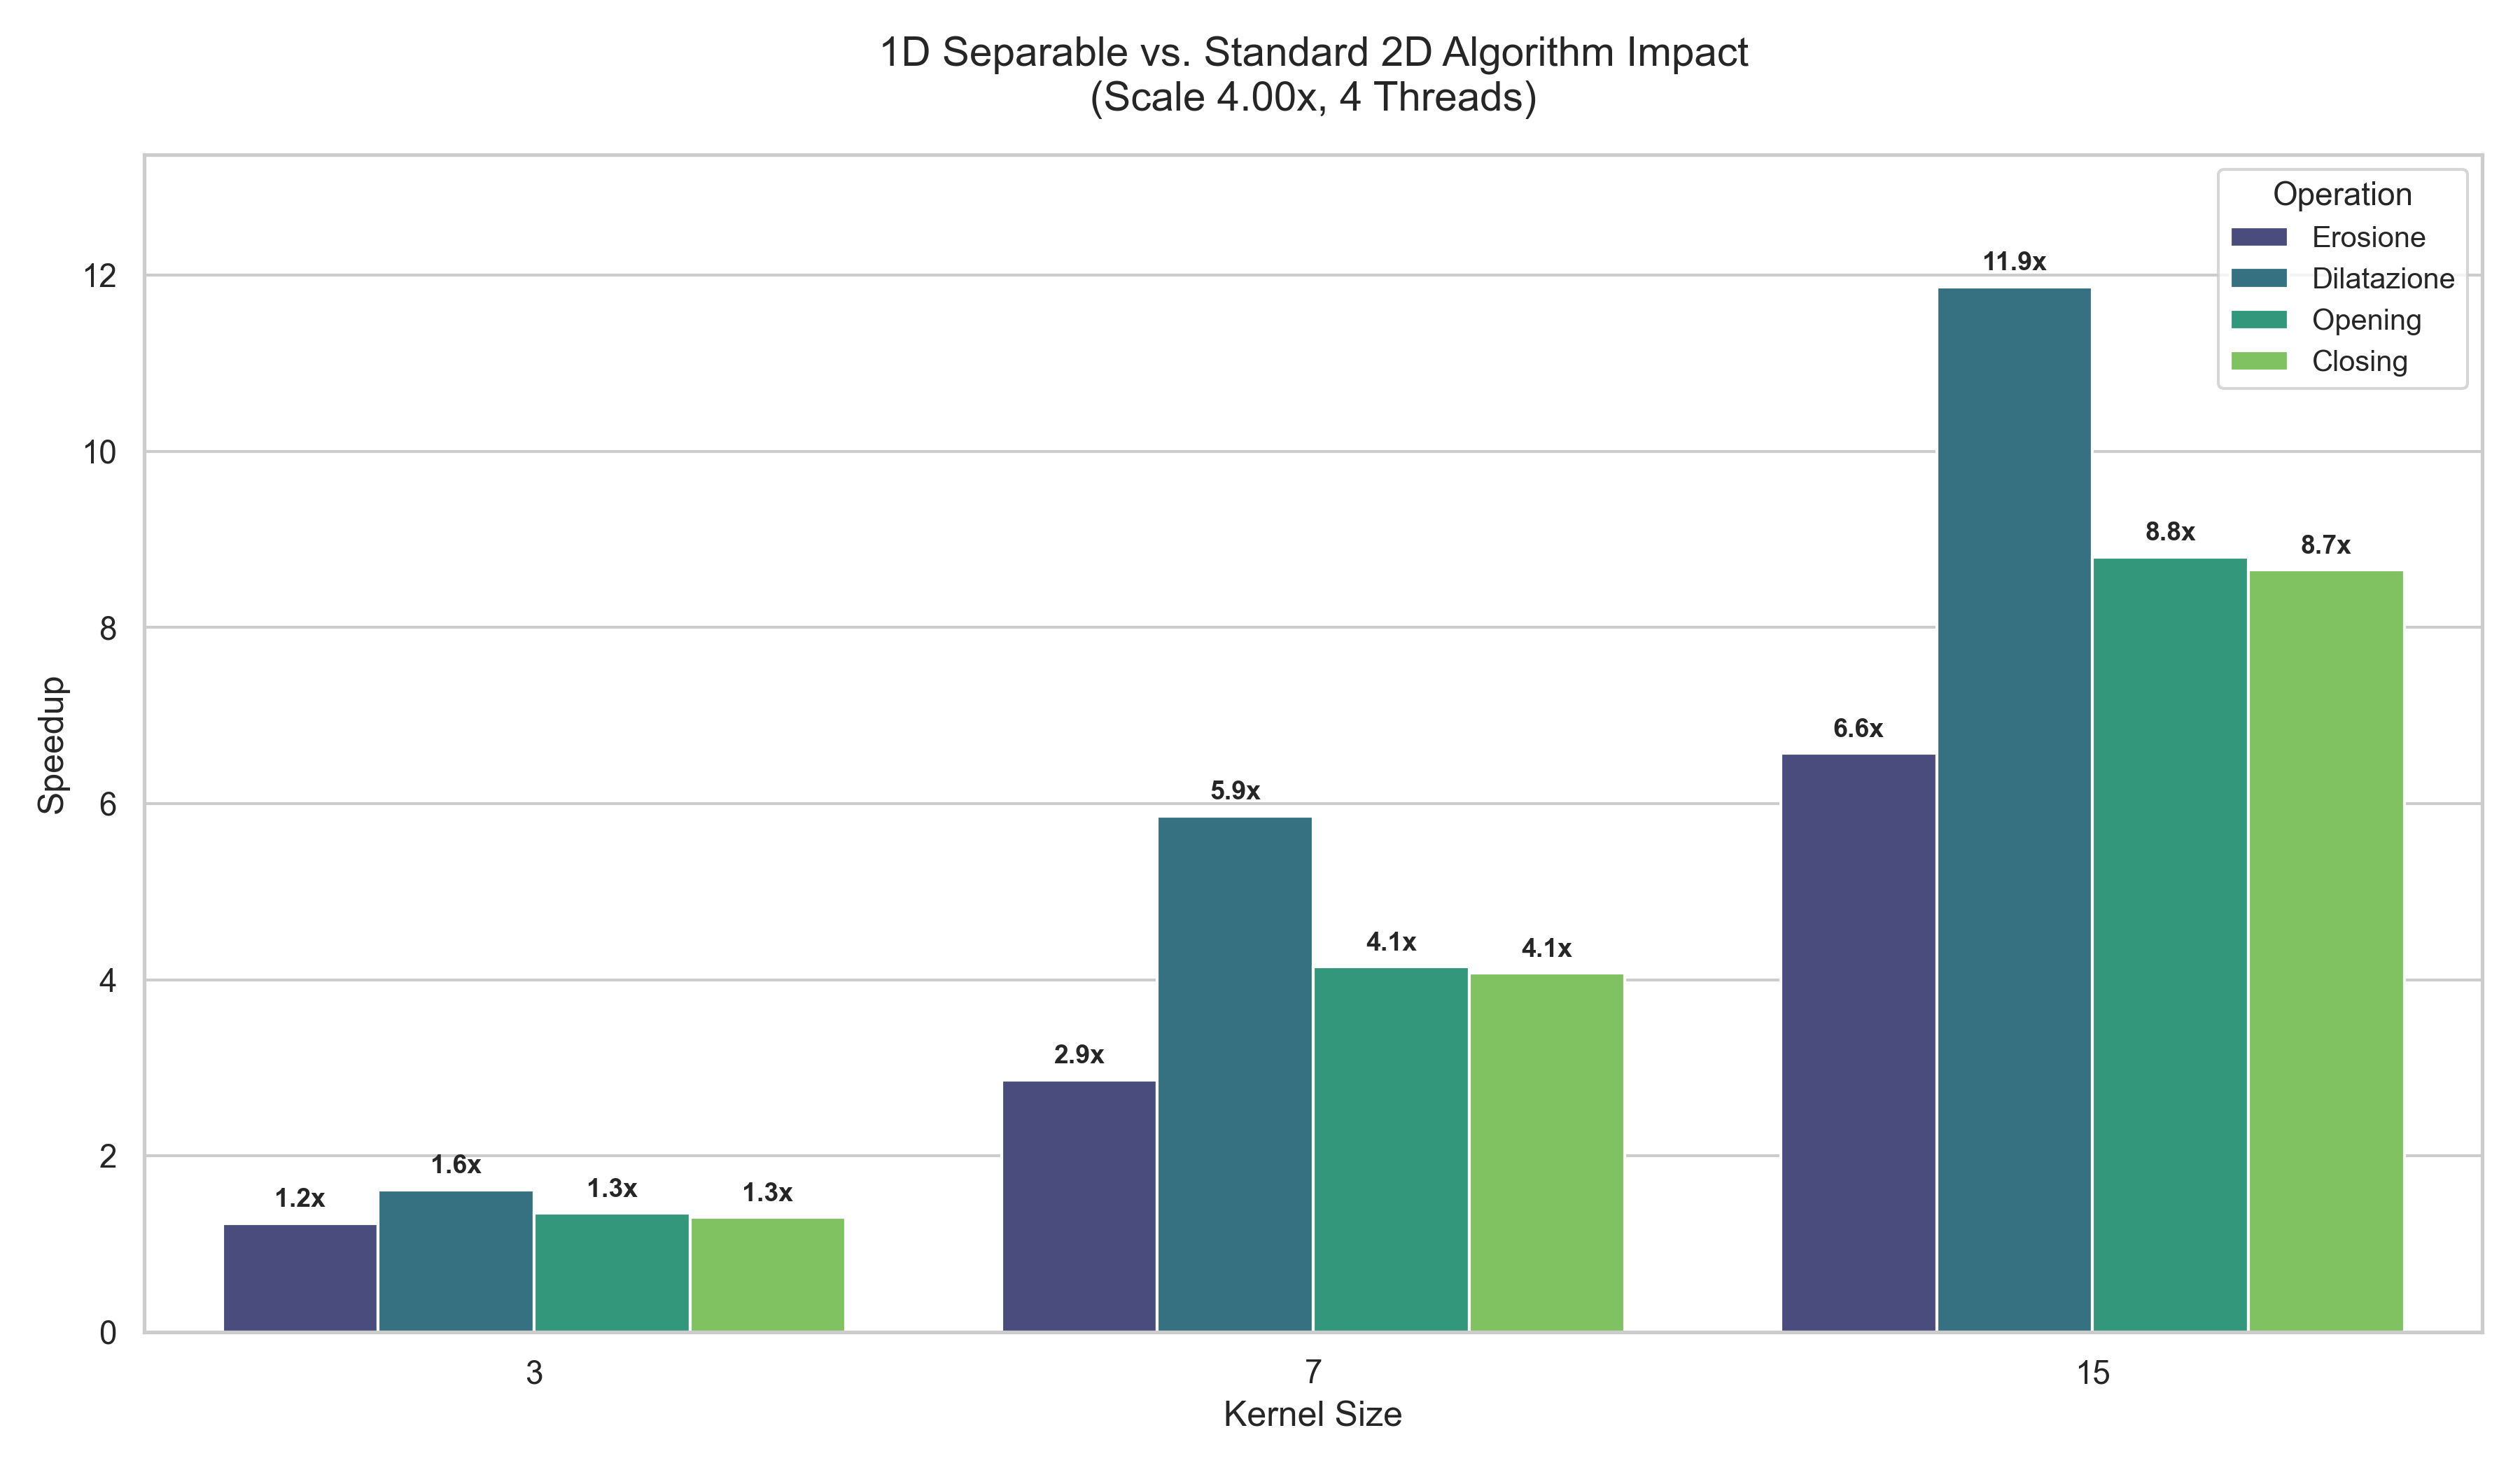
\includegraphics[width=\textwidth]{img/separable_speedup_scale_4.0x.png}
          \caption{Speedup of 1D Separable Kernels vs 2D baseline}
      \end{figure}
    \end{column}
  \end{columns}
\end{frame}

% --- SLIDE 9 ---
\begin{frame}{Producer-Consumer Pipeline Efficiency}
  \begin{columns}
    \begin{column}{0.45\textwidth}
      \begin{itemize}
        \item \textbf{Focus:} specific optimization for Opening and Closing
        \item \textbf{Peak Efficiency:} yields up to a \textbf{1.52x} performance boost over the standard parallel baseline
\item \textbf{High-Concurrency Contention:}
          \begin{itemize}
            \item Active \textit{spin-wait} loops saturate physical cores under high logical thread counts
            \item Cross-chunk dependencies amplify synchronization overhead and cause thread starvation
          \end{itemize}
      \end{itemize}
    \end{column}
    \begin{column}{0.5\textwidth}
      \begin{figure}
          \centering
          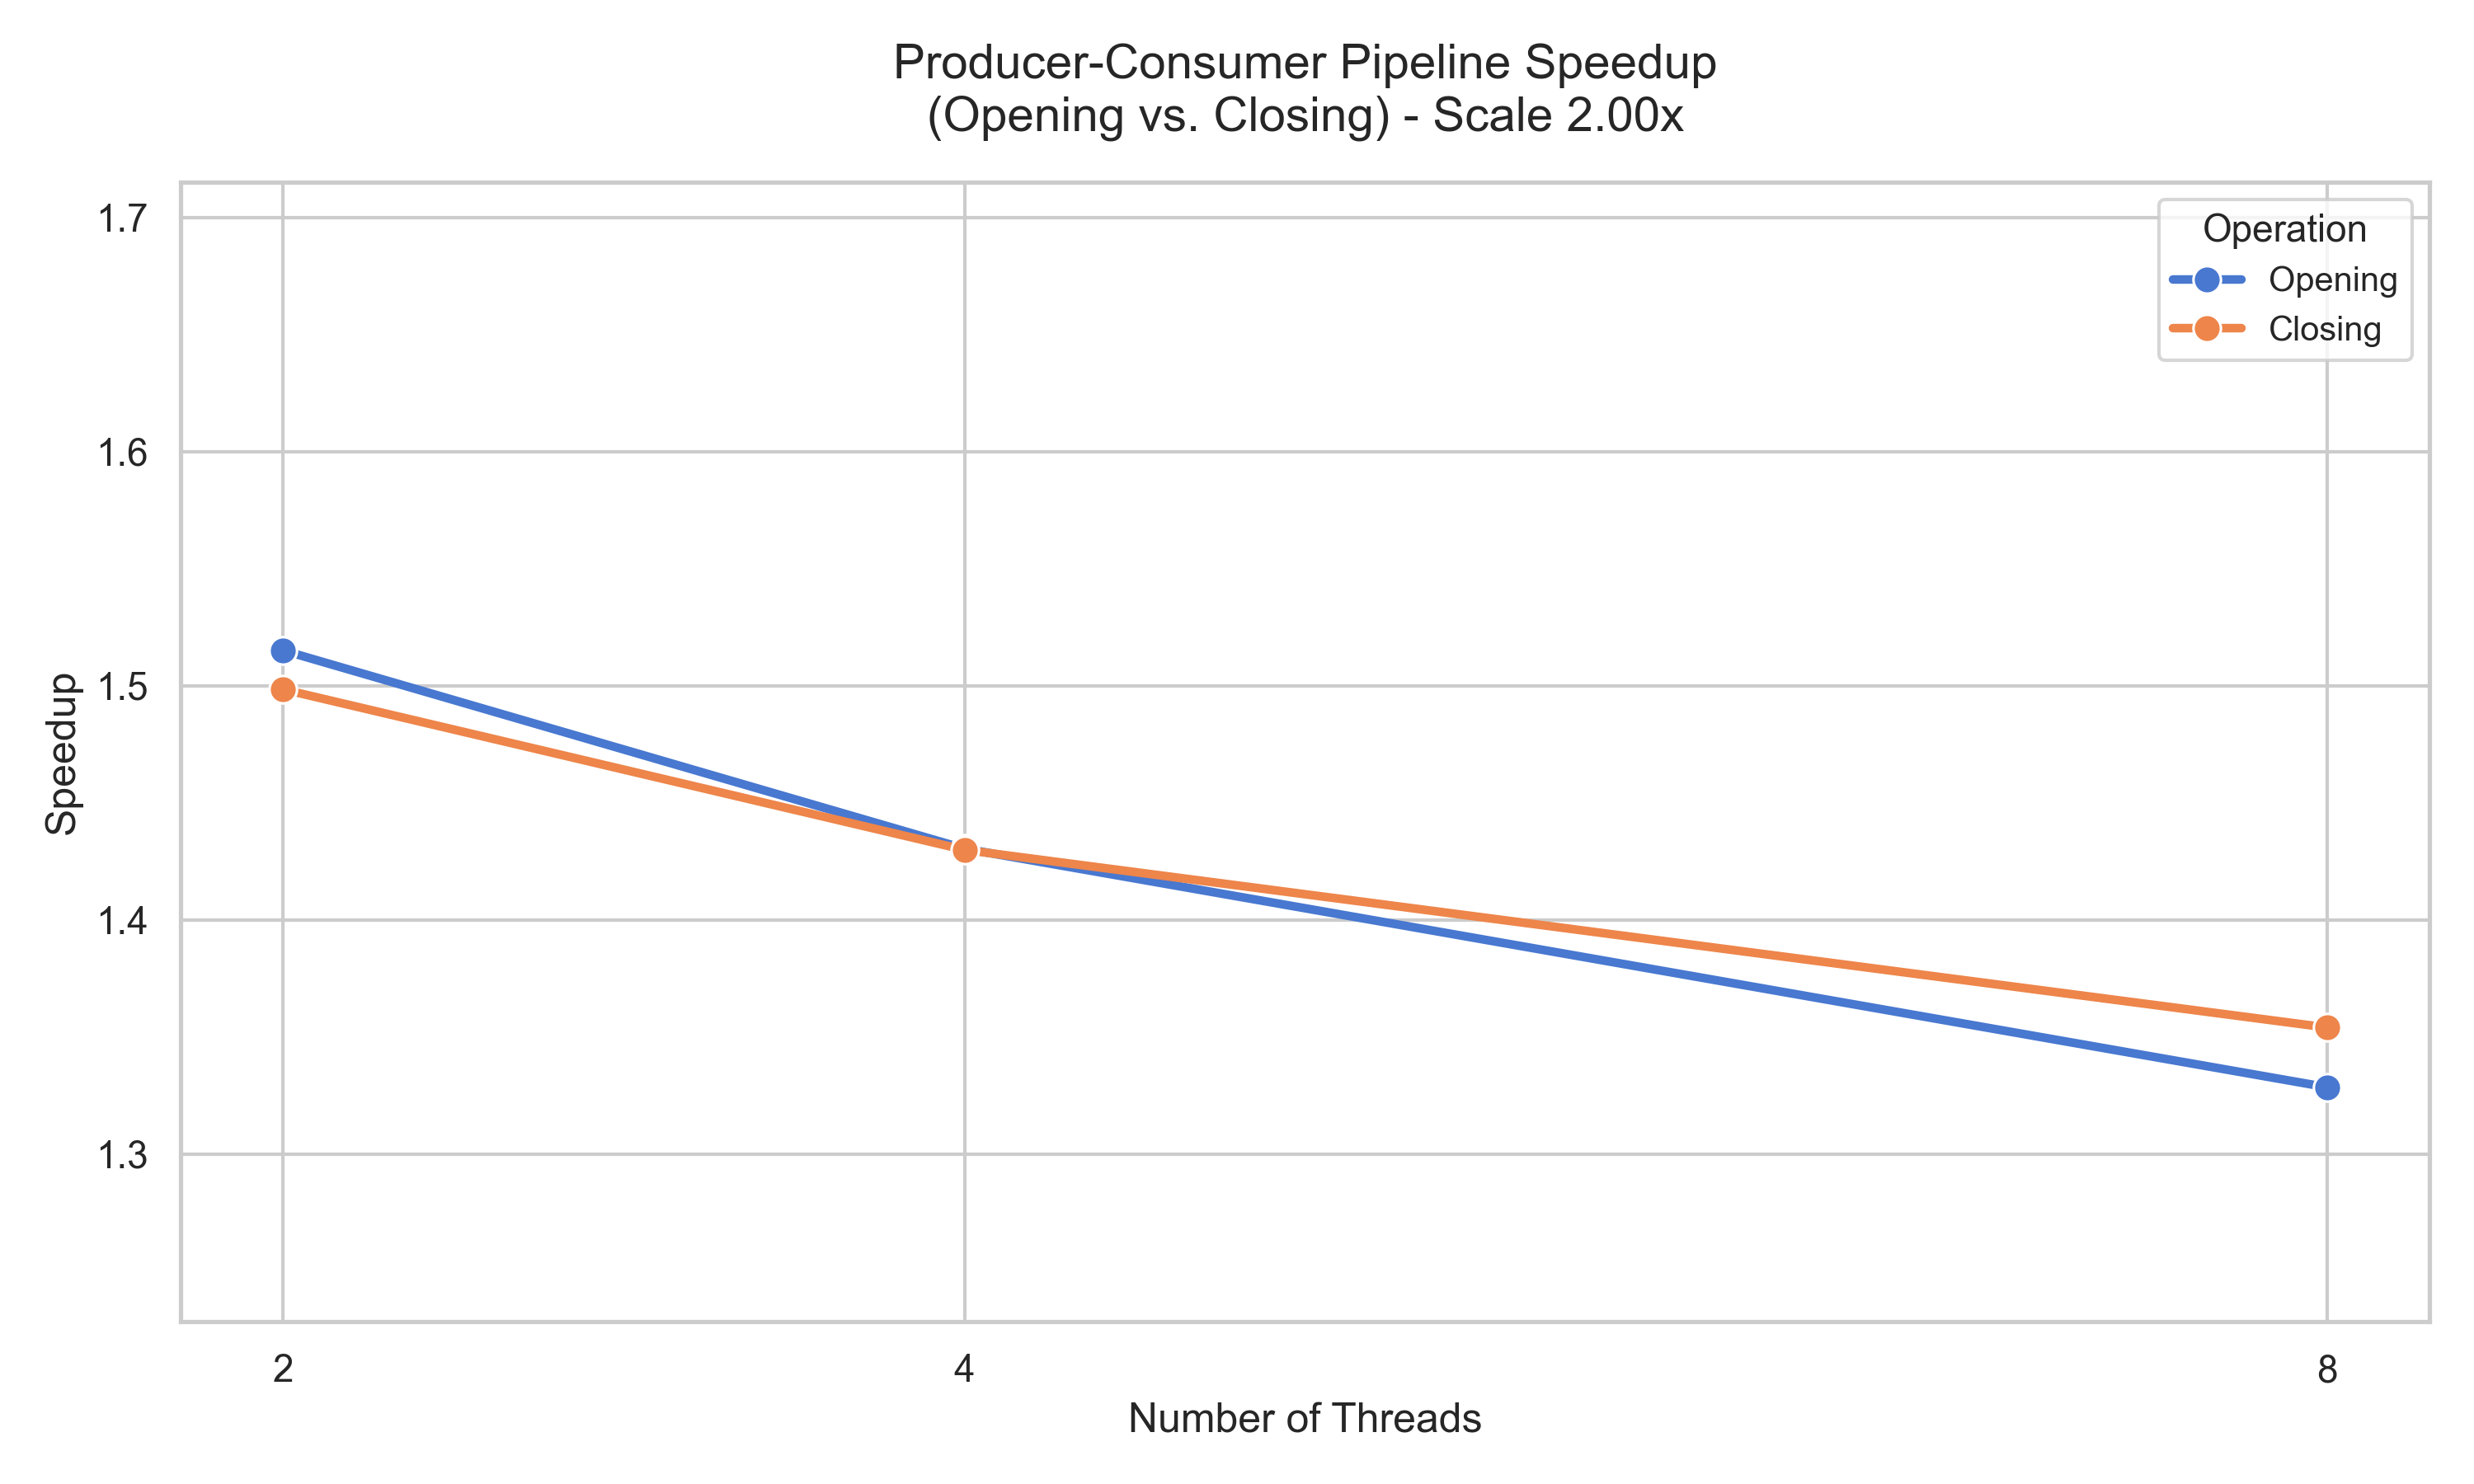
\includegraphics[width=\textwidth]{img/pipeline_speedup_scale_2.0x.png}
          \caption{Pipeline speedup for compound operations}
      \end{figure}
    \end{column}
  \end{columns}
\end{frame}


% --- SLIDE 10 ---
\begin{frame}{Other Strategies Tested}
  \begin{itemize}
    \item \textbf{SIMD Vectorization (\texttt{\#pragma omp simd}):}
      \begin{itemize}
        \item No positive impact on core loops
        \item Failure due to compiler auto-vectorization (already optimal) and min/max conditional branches
      \end{itemize}
    \vspace{0.3cm}
    \item \textbf{Dynamic Loop Scheduling (\texttt{schedule(dynamic)}):}
      \begin{itemize}
        \item Evaluated on the baseline parallel version to improve load balancing
        \item Performance remained virtually identical to the default \texttt{static} approach
      \end{itemize}
  \end{itemize}
\end{frame}

% --- SLIDE 11 ---
\begin{frame}{Peak Performance \& Future Developments}
  \begin{columns}
    \begin{column}{0.45\textwidth}
      \begin{colorblock}[white]{sintefblu1}{Optimal Configuration}
        \begin{center}
          \Large \textbf{22x Peak Speedup}
        \end{center}
        Mixed 1D Separable + OpenMP architecture ($K=15$, 4 Threads) over 2D Baseline.
      \end{colorblock}
    \end{column}
    \begin{column}{0.55\textwidth}
      \begin{itemize}
        \item \textbf{Hardware/Software Conclusion:} bare multithreading can't save a flawed algorithm. Hardware/software integration is the only path to raise high performance
        \item \textbf{Heterogeneous Computing (Future Work):}
          \begin{itemize}
            \item Porting the logic to GPU architectures (CUDA)
          \end{itemize}
      \end{itemize}
    \end{column}
  \end{columns}
\end{frame}

% --- SLIDE (Opzionale) ---
\begin{frame}{Visual Results}  
  \begin{columns}
    \begin{column}{0.33\textwidth}
      \centering
      \textbf{Original} \\
      \vspace{0.1cm}
      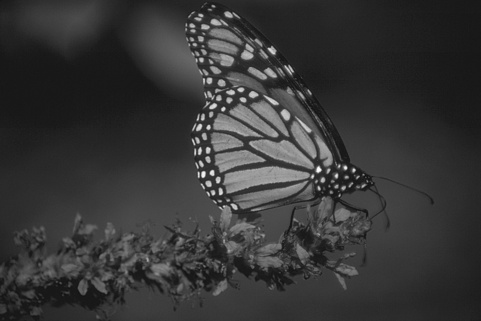
\includegraphics[width=0.9\textwidth]{img/original.png}
    \end{column}
    \begin{column}{0.33\textwidth}
      \centering
      \textbf{Erosion} \\
      \vspace{0.1cm}
      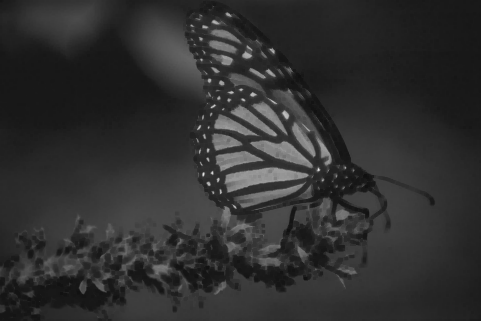
\includegraphics[width=0.9\textwidth]{img/eroded.png}
    \end{column}
    \begin{column}{0.33\textwidth}
      \centering
      \textbf{Dilation} \\
      \vspace{0.1cm}
      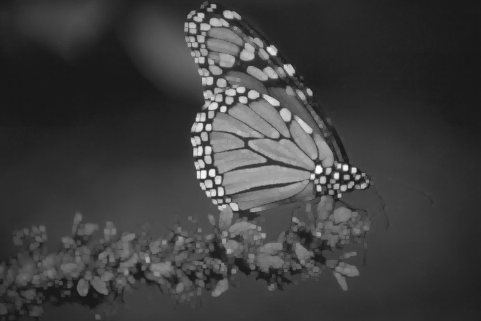
\includegraphics[width=0.9\textwidth]{img/dilated.png}
    \end{column}
  \end{columns}
  
  \vspace{0.4cm} 
  
  \begin{columns}
    \begin{column}{0.33\textwidth}
    \end{column}
    \begin{column}{0.33\textwidth}
      \centering
      \textbf{Opening} \\
      \vspace{0.1cm}
      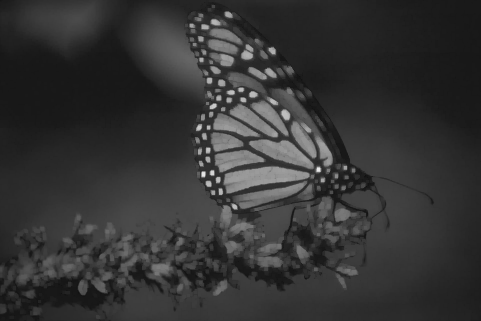
\includegraphics[width=0.9\textwidth]{img/opening.png}
    \end{column}
    \begin{column}{0.33\textwidth}
      \centering
      \textbf{Closing} \\
      \vspace{0.1cm}
      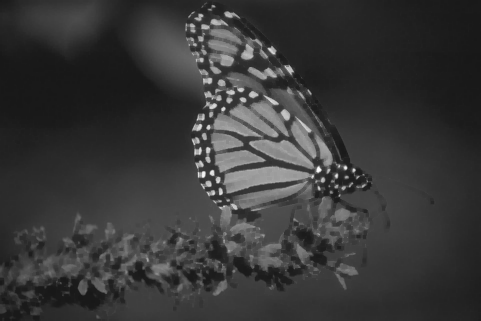
\includegraphics[width=0.9\textwidth]{img/closing.png}
    \end{column}
  \end{columns}
\end{frame}

\backmatter
\end{document}